%%%%%%%%%%%%%%%%%%%%%%%%%%%%%%%%%%%%%%%%%%%%%%%%%%%%%%%%%%%%%%%%%%%%%%%
%
%  Synthetic Surrealism
%
%

 
% Make two column format for LaTex 2e.
\documentclass{article}
\usepackage{times}

% Use following instead for LaTex 2.09 (may need some other mods as well).
% \documentstyle[times,twocolumn]{article}
% \usepackage[pdftex]{graphicx}

\usepackage{amssymb}
\usepackage{epsfig}
\usepackage{algorithm,algorithmic}
\usepackage{subfigure}

\pagestyle{empty}
                     



\def\A{{\cal A}}
\def\B{{\cal B}}
\def\C{{\cal C}}
\def\D{{\cal D}}
\def\E{{\cal E}}
\def\F{{\cal F}}
\def\J{{\cal J}}
\def\L{{\cal L}}
\def\M{{\cal M}}
\def\P{{\cal P}}
\def\Q{{\cal Q}}
\def\S{{\cal S}}
\def\V{{\cal V}}
\def\W{{\cal W}}
\def\X{{\cal X}}
\def\Y{{\cal Y}}
\def\SR{{\mathbb{R}}}
\def\MT{{\mathfrak{T}}}
\def\ME{{\mathfrak{E}}}
\def\MP{{\mathfrak{P}}}
\def\a{\alpha}
\def\e{{\bf e}}

\begin{document}

% Don't want date printed
\date{}


\title{Synthetic Surrealism }

\author{
Trip Denton  \\
        \emph{Synthetic Surrealism Group of Philadelphia}  %\\
}

 

\maketitle

\thispagestyle{empty}

\begin{abstract}

  
\end{abstract}
  
%%%%%%%%%%%%%%%%%%%%%%%%%%%%%%%%%%%%%%%%%%%%%%%%%%%%%%%%%%%%%%%%%%%%%%%%%%%%%%%
\section{Introduction \& Background}
\label{sec:intro}
%%%%%%%%%%%%%%%%%%%%%%%%%%%%%%%%%%%%%%%%%%%%%%%%%%%%%%%%%%%%%%%%%%%%%%%%%%%%%%%
\vspace{-0.1in}
Given a set of patterns

\begin{figure}[!ht]
        \centerline{
        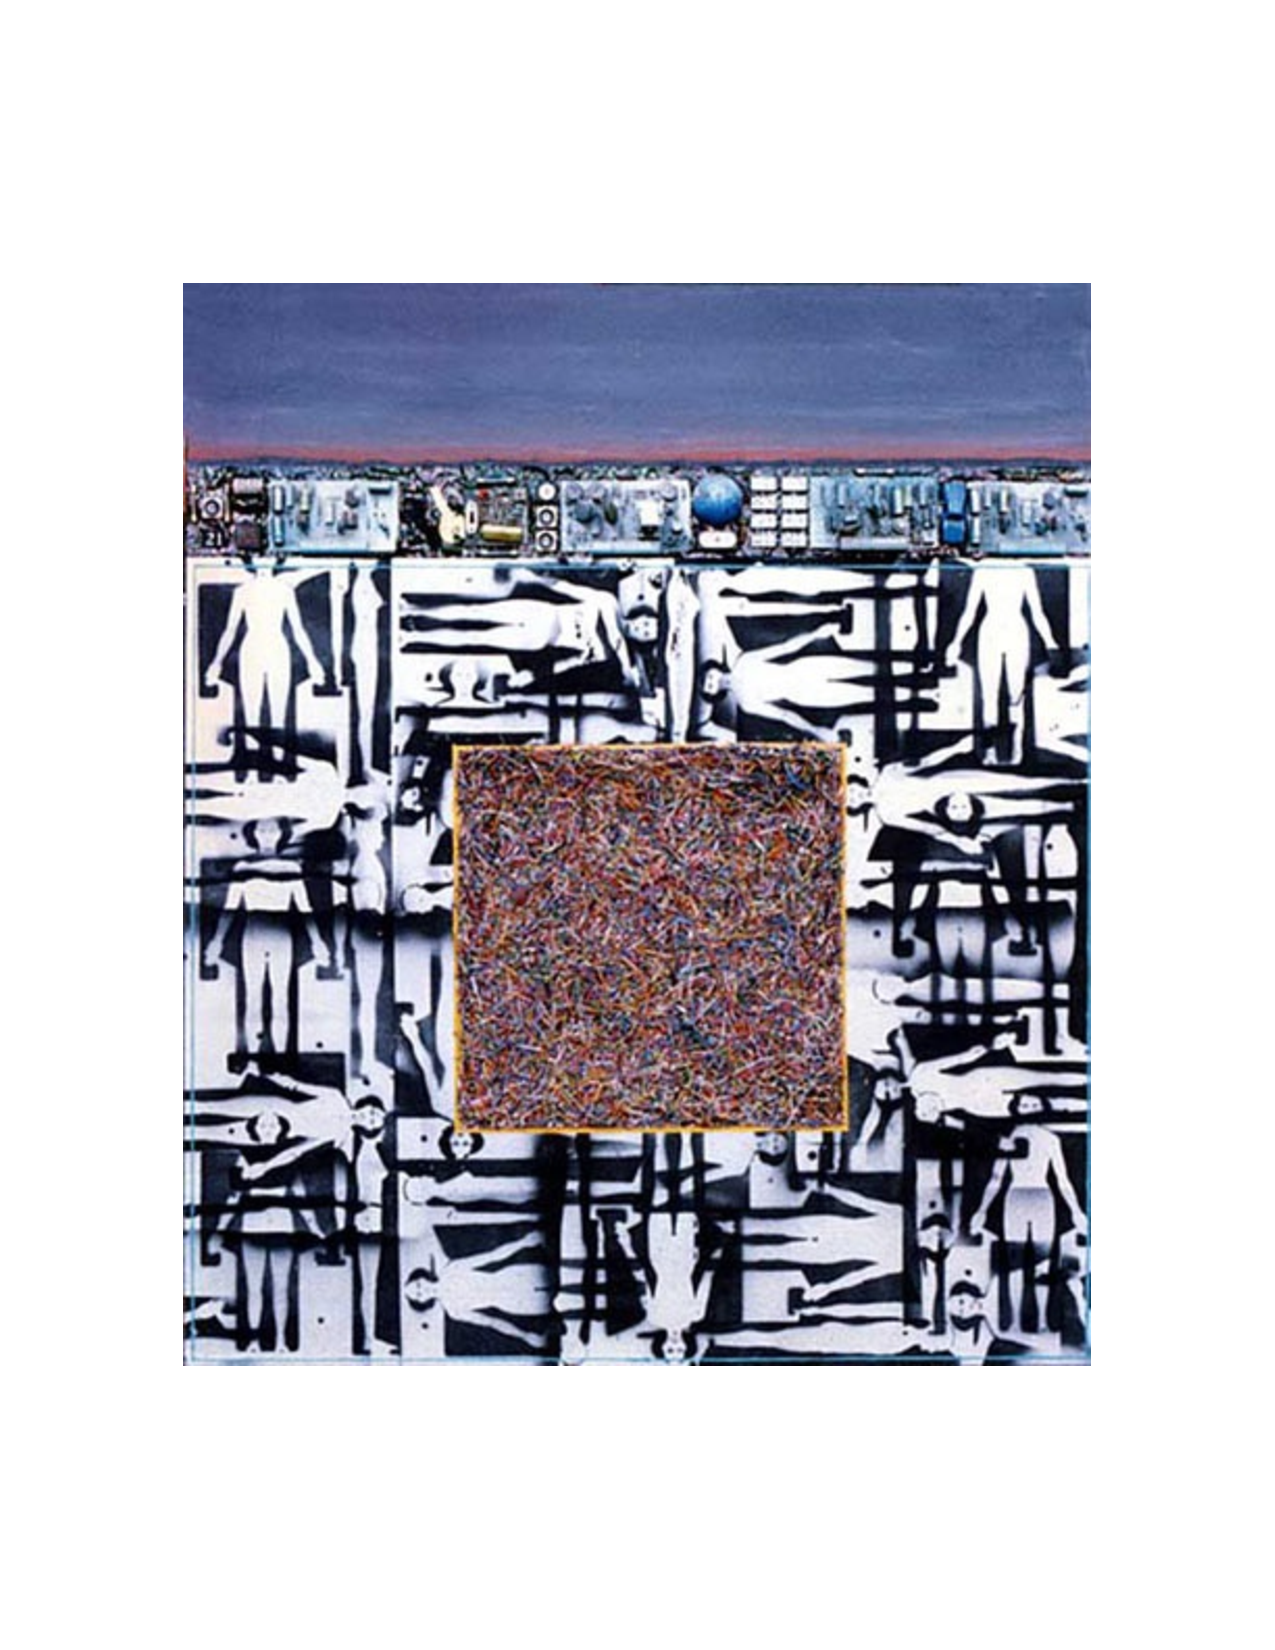
\includegraphics[scale=0.5]{img/h001.pdf} \\
   }
        \caption{Motivation: Given the 3D model in (a) and a  set
          of views in (b), and similarity function among the views,
          identify a small subset of views that best characterizes the
          object. The boxed views represent the canonical set obtained
          through our algorithm.}
        \label{fig:canset_motivation}
\end{figure}


                                        

In developing an approximation framework for computing canonical sets,

\vspace{-0.1in}
%%%%%%%%%%%%%%%%%%%%%%%%%%%%%%%%%%%%%%%%%%%%%%%%%%%%%%%%%%%%%%%%%%%%%%%%%%%%%%%
\section{Problem Formulation}
\label{sec:form}
%%%%%%%%%%%%%%%%%%%%%%%%%%%%%%%%%%%%%%%%%%%%%%%%%%%%%%%%%%%%%%%%%%%%%%%%%%%%%%%
%
\vspace{-0.1in}
In this section we define the notion of canonical set.  This
combinatoric problem is unfortunately intractable.  We therefore
present a series of steps (integer programming, quadratic programming,
semidefinite programming, and finally rounding) that allow us to
compute good approximate solutions in polynomial time.
\vspace{-0.1in}
\subsection{Definitions}
\vspace{-0.1in}

%%%%%%%%%%%%%%%%%%%%%%%%%%%%%%%%%%%%%%%
\section{Summary and Future Work}
\label{sec:conclusion}

%%%%%%%%%%%%%%%%%%%%%%%%%%%%%%%%%%%%%%%
\vspace{-0.1in}
We have developed an approximation framework for the canonical set
problem based on SDP relaxation of an integer programming formulation.
Through a series of experiments we evaluated this framework in the
context of 2D view simplification of 3D objects. Our results compared
favorably to exhaustive search.



\bibliographystyle{ieee}
\bibliography{tdenton}

\end{document}
